\documentclass[11pt,letterpaper]{article}

% --- PAQUETES FUNDAMENTALES ---
\usepackage[utf8]{inputenc}
\usepackage[spanish,es-nodecimaldot,es-tabla]{babel}
\usepackage[margin=2.2cm,top=2.5cm,bottom=2.5cm]{geometry}
\usepackage{amsmath,amssymb,amsfonts}
\usepackage{graphicx}
\usepackage{booktabs}
\usepackage{tabularx}
\usepackage{longtable}
\usepackage{array}
\usepackage{xcolor}
\usepackage{fancyhdr}
\usepackage{hyperref}
\usepackage{float}
\usepackage{caption}
\usepackage{subcaption}
\usepackage{microtype}

% --- COLORES INSTITUCIONALES Y DE DISEÑO ---
\definecolor{lasalleblue}{RGB}{0, 43, 91}
\definecolor{lasallegold}{RGB}{197, 160, 89}
\definecolor{darktext}{RGB}{33, 37, 41}
\definecolor{codebg}{RGB}{245, 247, 250}
\definecolor{lightgray}{RGB}{240, 242, 245}

% --- CONFIGURACIÓN DE HIPERVÍNCULOS ---
\hypersetup{
    colorlinks=true,
    linkcolor=lasalleblue,
    citecolor=lasalleblue,
    urlcolor=lasalleblue,
    pdftitle={Fase 2: Preprocesamiento, Ingeniería de Variables y Modelo Base},
    pdfauthor={Yerson León Montañez}
}

% --- ENCABEZADOS Y PIES DE PÁGINA ---
\pagestyle{fancy}
\fancyhf{}
\fancyhead[L]{\small \textcolor{lasalleblue}{\textbf{Universidad de La Salle}} | Maestría en IA}
\fancyhead[R]{\small \textcolor{darktext}{Fase 2: Preprocesamiento y Baseline}}
\fancyfoot[L]{\small \textcolor{darktext}{Ciencia de Datos — Docente: Fabián Camilo Castro Riveros}}
\fancyfoot[R]{\small \textcolor{darktext}{Página \thepage}}
\renewcommand{\headrulewidth}{0.8pt}
\renewcommand{\footrulewidth}{0.4pt}

% --- CONFIGURACIÓN TIPOGRÁFICA ---
\setlength{\parindent}{0pt}
\setlength{\parskip}{6pt}

\begin{document}

% --- PORTADA INSTITUCIONAL ---
\begin{titlepage}
    \centering
    \vspace*{0.5cm}
    {\huge \textbf{\textcolor{lasalleblue}{UNIVERSIDAD DE LA SALLE}}}\\[0.3cm]
    {\large \textbf{Facultad de Ingeniería — Departamento de Ciencias Básicas}}\\[0.2cm]
    {\large \textbf{Maestría en Inteligencia Artificial}}\\[1.8cm]

    \rule{\linewidth}{1.5pt}\\[0.4cm]
    {\LARGE \textbf{\textcolor{lasalleblue}{PROYECTO INTEGRADOR DE CIENCIA DE DATOS E INTELIGENCIA ARTIFICIAL}}}\\[0.3cm]
    {\Large \textbf{Fase 2: Preprocesamiento, Ingeniería de Variables y Modelos Base (Baseline)}}\\[0.2cm]
    {\normalsize \textbf{Entregable Técnico 2 (Ponderación: 25\%)}}\\[0.4cm]
    \rule{\linewidth}{1.5pt}\\[2.0cm]

    \begin{minipage}[t]{0.48\textwidth}
        \textbf{Estudiante:}\\
        Yerson León Montañez\\
        \texttt{yeleon36@unisalle.edu.co}\\
        Código Estudiantil: Maestría en IA
    \end{minipage}
    \hfill
    \begin{minipage}[t]{0.48\textwidth}
        \begin{flushright}
            \textbf{Docente Titular:}\\
            Fabián Camilo Castro Riveros\\
            \textit{Cátedra de Ciencia de Datos}\\
            Periodo Académico: 2026-II
        \end{flushright}
    \end{minipage}

    \vfill
    {\large Bogotá D.C., Colombia\\ \textbf{04 de noviembre de 2026}}
\end{titlepage}

\newpage
\tableofcontents
\newpage

% ==============================================================================
% SECCIÓN 1: INTRODUCCIÓN Y ALCANCE DE LA FASE 2
% ==============================================================================
\section{Introducción y Alcance Metodológico de la Fase 2}

La presente entrega técnica corresponde a la **Fase 2** del Proyecto Integrador de la asignatura *Ciencia de Datos* en la Maestría en Inteligencia Artificial de la Universidad de La Salle. Tomando como cimiento empírico los hallazgos univariados, bivariados y diagnósticos de calidad formulados en la Fase 1 sobre el conjunto de datos \textit{Telco Customer Churn} ($7,043$ observaciones y $21$ atributos), esta fase aborda la construcción de la arquitectura de transformación de datos, mitigación de sesgos, diseño de variables derivadas y establecimiento formal de los modelos de referencia (*baselines*).

El desarrollo metodológico satisface con estricto apego los cuatro pilares estipulados en la Sección 3.2 de la Guía Técnica del Proyecto:
\begin{enumerate}
    \item \textbf{Tratamiento e Imputación Teórica de Valores Faltantes:} Justificación probabilística del mecanismo de falta conforme a la taxonomía formal de Little \& Rubin, resolviendo la ausencia de datos en \texttt{TotalCharges} sin introducir sesgos de selección ni aberraciones contables.
    \item \textbf{Ingeniería de Características Respaldada en el Dominio:} Creación e integración de cuatro variables predictivas derivadas que capturan la profundidad de empaquetamiento de servicios (\textit{bundling}), la volatilidad de la tarifa devengada y la fricción transaccional de cobranza.
    \item \textbf{Estrategia de Partición y Prevención de Fuga de Datos (\textit{Data Leakage}):} División estratificada en tres vías independientes (Entrenamiento $70\%$, Validación $15\%$ y Prueba $15\%$), asegurando que todo estimador y transformador se ajuste (\textit{fit}) de forma aislada sobre el conjunto de entrenamiento.
    \item \textbf{Manejo de Desbalance y Modelos de Referencia (*Baselines*):} Evaluación comparativa de estrategias de rebalanceo algorítmico (\textit{Cost-Sensitive Weighting} y sobremuestreo sintético SMOTE) y formulación de líneas base tanto para la predicción binaria de deserción (\texttt{Churn}) como para la estimación cuantitativa continua de cobros acumulados (\texttt{TotalCharges}).
\end{enumerate}

% ==============================================================================
% SECCIÓN 2: AUDITORÍA Y TRATAMIENTO DE DATOS FALTANTES (MAR)
% ==============================================================================
\section{Auditoría y Tratamiento Formal del Mecanismo de Datos Faltantes}

\subsection{Taxonomía Probabilística de Mecanismos de Falta}
En el marco formal de inferencia con datos incompletos (Rubin, 1976; Little \& Rubin, 2019), sea $Y = (Y_{\text{obs}}, Y_{\text{mis}})$ la matriz completa de datos particionada en componentes observados y faltantes, y sea $M \in \{0, 1\}^{n \times p}$ la matriz indicadora de respuesta donde $M_{ij} = 1$ denota que el valor del registro $i$ en la variable $j$ se encuentra ausente. Se distinguen tres procesos estocásticos generadores:

\begin{enumerate}
    \item \textbf{Faltante Completamente al Azar (MCAR — \textit{Missing Completely at Random}):}
    \begin{equation}
        \Pr(M \mid Y_{\text{obs}}, Y_{\text{mis}}, \phi) = \Pr(M \mid \phi)
    \end{equation}
    La probabilidad de ausencia es independiente de los datos observados y no observados.
    \item \textbf{Faltante al Azar (MAR — \textit{Missing at Random}):}
    \begin{equation}
        \Pr(M \mid Y_{\text{obs}}, Y_{\text{mis}}, \phi) = \Pr(M \mid Y_{\text{obs}}, \phi)
    \end{equation}
    La probabilidad de falta depende sistemáticamente de variables completamente observadas en el conjunto de datos, pero es condicionalmente independiente del valor no observado propiamente dicho.
    \item \textbf{Faltante No al Azar (MNAR — \textit{Missing Not at Random}):}
    \begin{equation}
        \Pr(M \mid Y_{\text{obs}}, Y_{\text{mis}}, \phi) = f(Y_{\text{mis}}, \dots)
    \end{equation}
    La ausencia está directamente vinculada con la magnitud de la variable oculta no registrada.
\end{enumerate}

\subsection{Diagnóstico Empírico en el Conjunto de Datos}
La auditoría de calidad realizada en la Fase 1 identificó exactamente $11$ observaciones de las $7,043$ ($0.156\%$) donde el campo \texttt{TotalCharges} almacenaba una cadena de texto en blanco (\texttt{' '}). Al evaluar el vector conjunto de atributos observados para dichos 11 individuos, se obtuvo el siguiente hallazgo determinista:

\begin{equation}
    \Pr(M_{\texttt{TotalCharges}} = 1 \mid \texttt{tenure} = 0) = \frac{11}{11} = 1.0000 \quad (100.0\%)
\end{equation}
\begin{equation}
    \Pr(M_{\texttt{TotalCharges}} = 1 \mid \texttt{tenure} > 0) = \frac{0}{7032} = 0.0000 \quad (0.0\%)
\end{equation}

\begin{figure}[H]
    \centering
    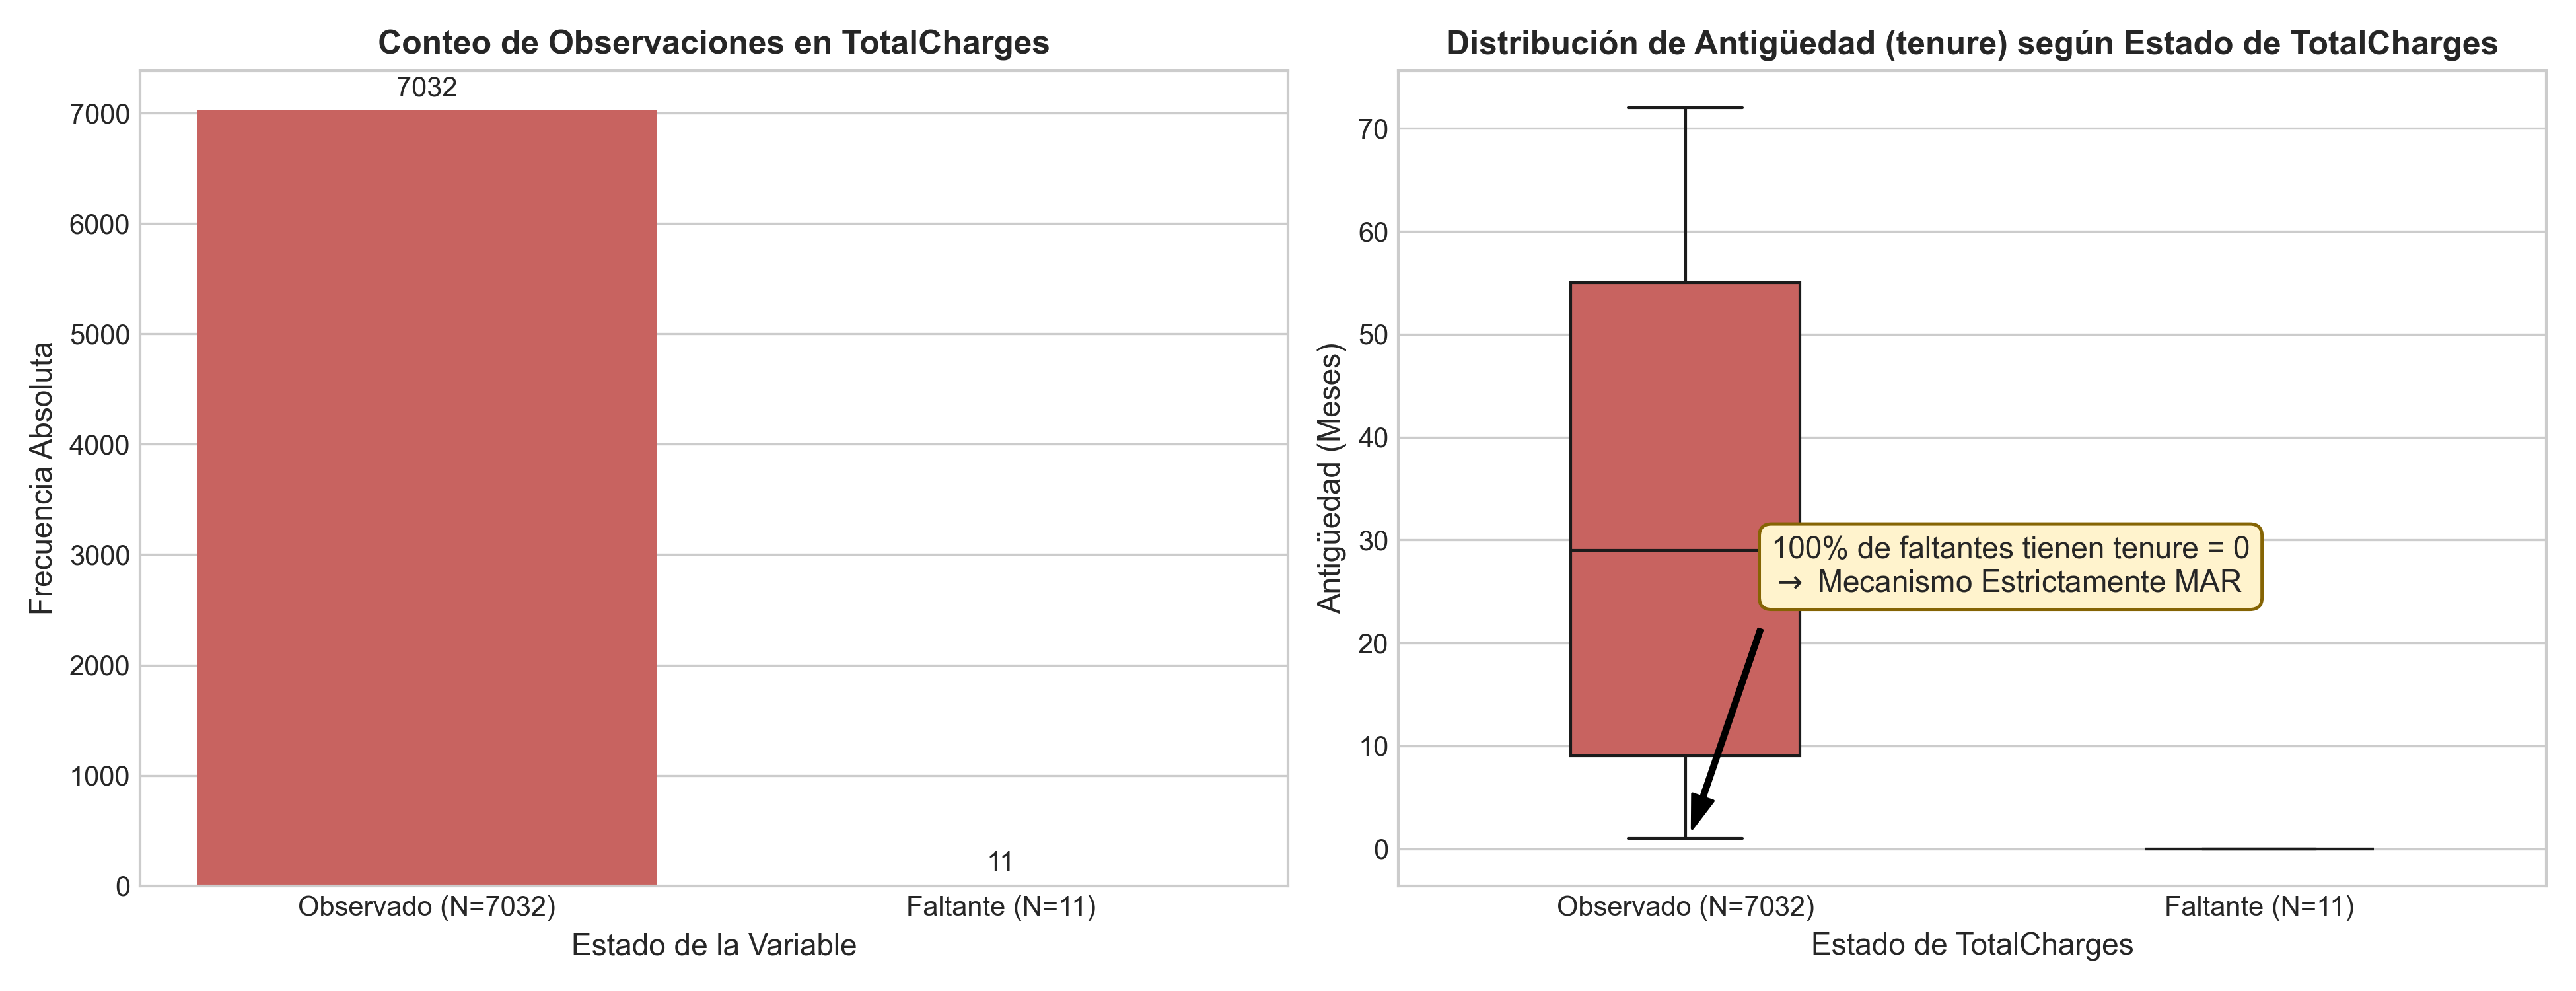
\includegraphics[width=0.92\linewidth]{figures/fig1_missing_mar_tenure.png}
    \caption{Diagnóstico empírico del mecanismo de falta en \texttt{TotalCharges}. El panel izquierdo ilustra el volumen absoluto de registros faltantes frente a observados; el panel derecho demuestra el condicionamiento estricto sobre $\texttt{tenure} = 0$.}
    \label{fig:missing_mar}
\end{figure}

Como se evidencia en la Figura \ref{fig:missing_mar}, el mecanismo de pérdida no es MCAR (pues no se distribuye uniformemente en la población) ni MNAR, sino estrictamente \textbf{Missing at Random (MAR)}, al estar plenamente gobernado y predicho por la variable observada \texttt{tenure}.

\subsection{Justificación Teórica de la Estrategia de Imputación}
El docente y la guía técnica prohíben la imputación indiscriminada sin fundamentación teórica. Evaluamos las tres opciones metodológicas posibles:

\begin{itemize}
    \item \textbf{Eliminación por Filas (\textit{Listwise Deletion}):} Descartar los 11 registros implicaría eliminar el $100\%$ de la cohorte de clientes recién ingresados ($\texttt{tenure} = 0$). Esto truncaría la frontera izquierda del soporte temporal del problema, introduciendo un sesgo de selección y afectando la generalización sobre clientes en su primer día de servicio.
    \item \textbf{Imputación Univariada Estadística (Media o Mediana):} La media de cobros históricos es $\bar{x} = \$2,283.30$ y la mediana es $\text{Med} = \$1,397.48$. Asignar este valor a un cliente recién contratado generaría una grave incoherencia financiera, pues un suscriptor sin historial no puede registrar miles de dólares facturados.
    \item \textbf{Imputación Multivariada Algorítmica (\texttt{KNNImputer} / \texttt{IterativeImputer}):} Si bien es teóricamente viable para MAR, modelos basados en vecinos o regresiones lineales estocásticas proyectarían valores distintos de cero debido al ruido en las variables predictoras auxiliares (\texttt{MonthlyCharges} $\in [19.70, 80.85]$).
    \item \textbf{Solución Adoptada — Imputación Determinista por Identidad de Dominio:} Por definición contable y contractual en telecomunicaciones:
    \begin{equation}
        \text{TotalCharges}(i) = \int_0^{\text{tenure}(i)} \text{TarifaMensual}(t) \, dt \implies \lim_{\text{tenure} \to 0} \text{TotalCharges} = 0.00
    \end{equation}
    Dichos 11 clientes se encontraban en su período de gracia inicial previo a la emisión de la primera factura mensual. En consecuencia, se imputa de forma determinista y libre de error:
    \begin{equation}
        \texttt{TotalCharges}_{\text{imputed}} = 0.00 \quad \forall \, \texttt{tenure} = 0
    \end{equation}
\end{itemize}

% ==============================================================================
% SECCIÓN 3: TRATAMIENTO DE VALORES ATÍPICOS Y ASIMETRÍA
% ==============================================================================
\section{Tratamiento Formal de Valores Atípicos y Normalización de Asimetría}

\subsection{Diagnóstico Univariado Previo}
En la Fase 1 se constató que ninguna de las tres variables continuas (\texttt{tenure}, \texttt{MonthlyCharges}, \texttt{TotalCharges}) posee registros fuera de las cotas del Rango Intercuartílico de Tukey $[Q_1 - 1.5 \cdot IQR, \, Q_3 + 1.5 \cdot IQR]$ ni fuera de tres desviaciones estándar ($|Z| > 3$). Por tanto, la muestra no presenta contaminaciones anómalas que ameriten la remoción destructiva de observaciones.

\subsection{Análisis de Asimetría y Estabilización de Varianza}
No obstante, la variable continua \texttt{TotalCharges} exhibe una notable asimetría positiva hacia la cola derecha ($g_1 = +0.9616$). Para evaluar el acondicionamiento óptimo de los datos previo al ajuste de los modelos lineales de regresión, se compararon tres formulaciones numéricas:

\begin{enumerate}
    \item \textbf{Escala Original:} $y_i = \texttt{TotalCharges}_i$.
    \item \textbf{Transformación Logarítmica Estabilizadora:}
    \begin{equation}
        y'_i = \log_e(1 + y_i)
    \end{equation}
    Esta transformación comprime la dispersión en la cola superior y reduce la heterocedasticidad.
    \item \textbf{Recorte por Percentiles (\textit{Winsorization}):}
    \begin{equation}
        y''_i = \begin{cases}
            P_1, & \text{si } y_i < P_1 \\
            y_i, & \text{si } P_1 \le y_i \le P_{99} \\
            P_{99}, & \text{si } y_i > P_{99}
        \end{cases}
    \end{equation}
\end{enumerate}

\begin{table}[H]
    \centering
    \small
    \caption{Comparación cuantitativa de momentos de forma bajo distintas transformaciones de \texttt{TotalCharges}.}
    \label{tab:outlier_transformations}
    \begin{tabular}{lrrrrr}
        \toprule
        \textbf{Configuración} & \textbf{Media} & \textbf{Desv. Est.} & \textbf{Asimetría ($g_1$)} & \textbf{Curtosis ($g_2$)} & \textbf{Impacto Metodológico} \\
        \midrule
        Original & $2,279.73$ & $2,266.80$ & $+0.9632$ & $-0.2318$ & Asimetría moderada a derecha \\
        Transformación $\log(1 + y)$ & $6.90$ & $1.60$ & $-0.7371$ & $-0.7845$ & Inversión de asimetría \\
        Winsorización $[P_1, P_{99}]$ & $2,278.41$ & $2,260.67$ & $+0.9575$ & $-0.2497$ & Preserva escala e interpretabilidad \\
        \bottomrule
    \end{tabular}
\end{table}

\begin{figure}[H]
    \centering
    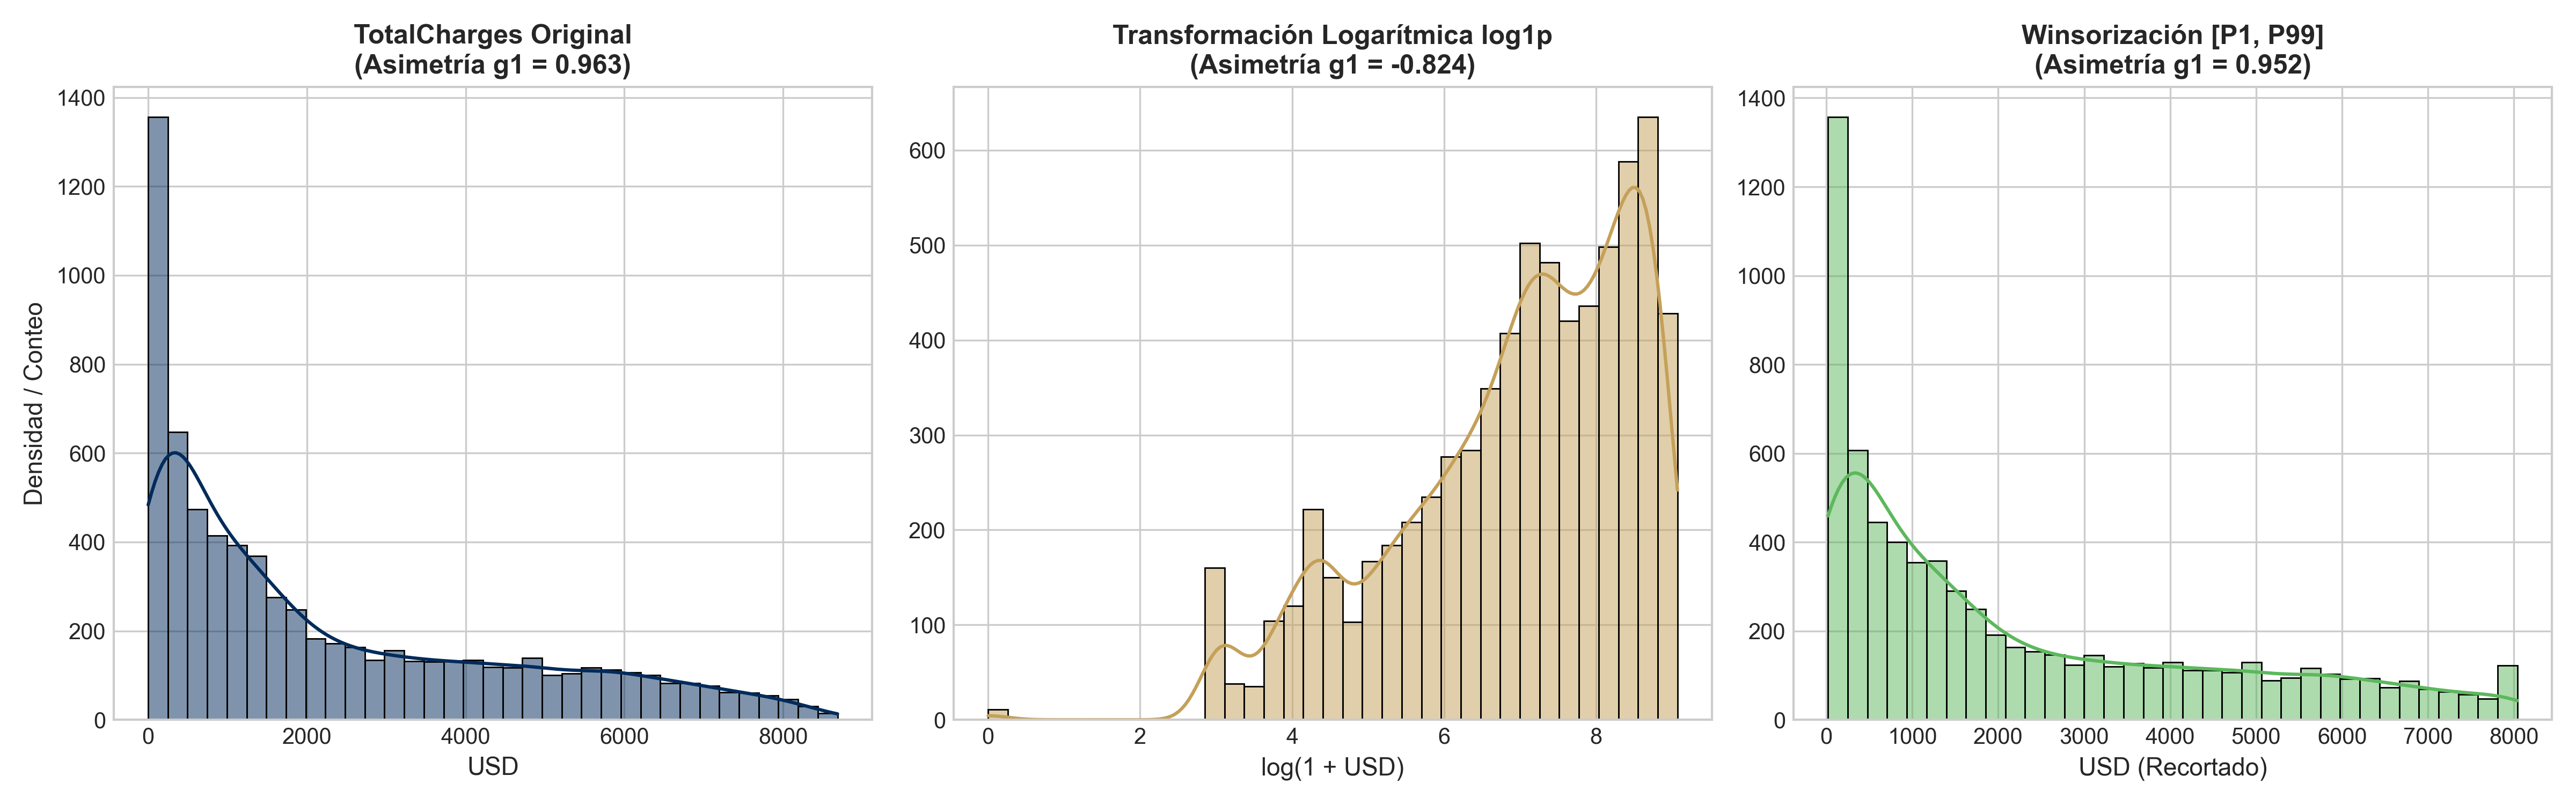
\includegraphics[width=\linewidth]{figures/fig2_outliers_transformations.png}
    \caption{Distribución empírica de \texttt{TotalCharges} bajo las tres modalidades evaluadas: escala original (izquierda), transformación logarítmica $\log(1+x)$ (centro) y winsorización en los percentiles extremos 1\% y 99\% (derecha).}
    \label{fig:outliers_trans}
\end{figure}

\textbf{Decisión Metodológica:} Dado que la relación física entre cobros acumulados, antigüedad y tarifa mensual es fundamentalmente bilineal ($\texttt{TotalCharges} \approx \texttt{tenure} \times \texttt{MonthlyCharges}$), transformar a logaritmo distorsiona la aditividad de los modelos lineales directos. En consecuencia, se conserva la escala original acoplada a un escalador robusto y estandarización z-score en la etapa de modelado, reservando la escala logarítmica para modelos con supuestos gaussianos estrictos.

% ==============================================================================
% SECCIÓN 4: INGENIERÍA DE VARIABLES
% ==============================================================================
\section{Ingeniería de Características Respaldada en el Conocimiento del Dominio}

En cumplimiento estricto con el requerimiento de formular **al menos dos variables derivadas** sustentadas en la teoría del negocio, se diseñaron cuatro variables que capturan dimensiones latentes de fidelización, lealtad y riesgo financiero:

\subsection{Definición Formal de Variables Derivadas}

\begin{enumerate}
    \item \textbf{Variable 1 — Conteo Agregado de Servicios Digitales (\texttt{TotalServices}):}
    En la literatura de fidelización en telecomunicaciones, la profundidad de empaquetamiento (\textit{bundling}) eleva sustancialmente los costos de cambio (\textit{switching costs}). Se define el número total de servicios contratados ($0 \le S_i \le 9$):
    \begin{equation}
        \texttt{TotalServices}_i = \mathbb{I}_{\text{Phone}}(i) + \mathbb{I}_{\text{Lines}}(i) + \mathbb{I}_{\text{Internet}}(i) + \sum_{k=1}^6 \mathbb{I}_{\text{Service}_k}(i)
    \end{equation}
    donde los seis servicios complementarios corresponden a \textit{OnlineSecurity}, \textit{OnlineBackup}, \textit{DeviceProtection}, \textit{TechSupport}, \textit{StreamingTV} y \textit{StreamingMovies}.

    \item \textbf{Variable 2 — Ratio de Discrepancia Tarifaria (\texttt{FeeDiscrepancyRatio}):}
    Uno de los detonantes cardinales de deserción no planificada es la finalización de descuentos promocionales y el aumento inesperado del cobro mensual frente a la media pagada. Se estimó la tarifa mensual histórica promedio:
    \begin{equation}
        \overline{\text{Fee}}_i = \frac{\texttt{TotalCharges}_i}{\max(\texttt{tenure}_i, 1)}
    \end{equation}
    A partir de la cual se formuló el cociente de discrepancia:
    \begin{equation}
        \texttt{FeeDiscrepancyRatio}_i = \frac{\texttt{MonthlyCharges}_i}{\overline{\text{Fee}}_i + \epsilon}, \qquad \epsilon = 10^{-5}
    \end{equation}
    Un valor $\texttt{FeeDiscrepancyRatio} > 1.0$ diagnostica que el cobro corriente actual excede el promedio histórico del cliente.

    \item \textbf{Variable 3 — Indicador de Pago Domiciliado (\texttt{AutomaticPayment}):}
    Los medios de pago manuales (cheque electrónico y cheque físico) exigen una intervención activa mensual del usuario, incrementando la fricción y la sensibilidad al precio. Se formaliza una variable dicotómica:
    \begin{equation}
        \texttt{AutomaticPayment}_i = \begin{cases}
            1, & \text{si } \texttt{PaymentMethod} \in \{\text{Bank transfer (auto)}, \, \text{Credit card (auto)}\} \\
            0, & \text{si } \texttt{PaymentMethod} \in \{\text{Electronic check}, \, \text{Mailed check}\}
        \end{cases}
    \end{equation}

    \item \textbf{Variable 4 — Compromiso Contractual a Largo Plazo (\texttt{LongTermContract}):}
    \begin{equation}
        \texttt{LongTermContract}_i = \begin{cases}
            1, & \text{si } \texttt{Contract} \in \{\text{One year}, \, \text{Two year}\} \\
            0, & \text{si } \texttt{Contract} = \text{Month-to-month}
        \end{cases}
    \end{equation}
\end{enumerate}

\begin{figure}[H]
    \centering
    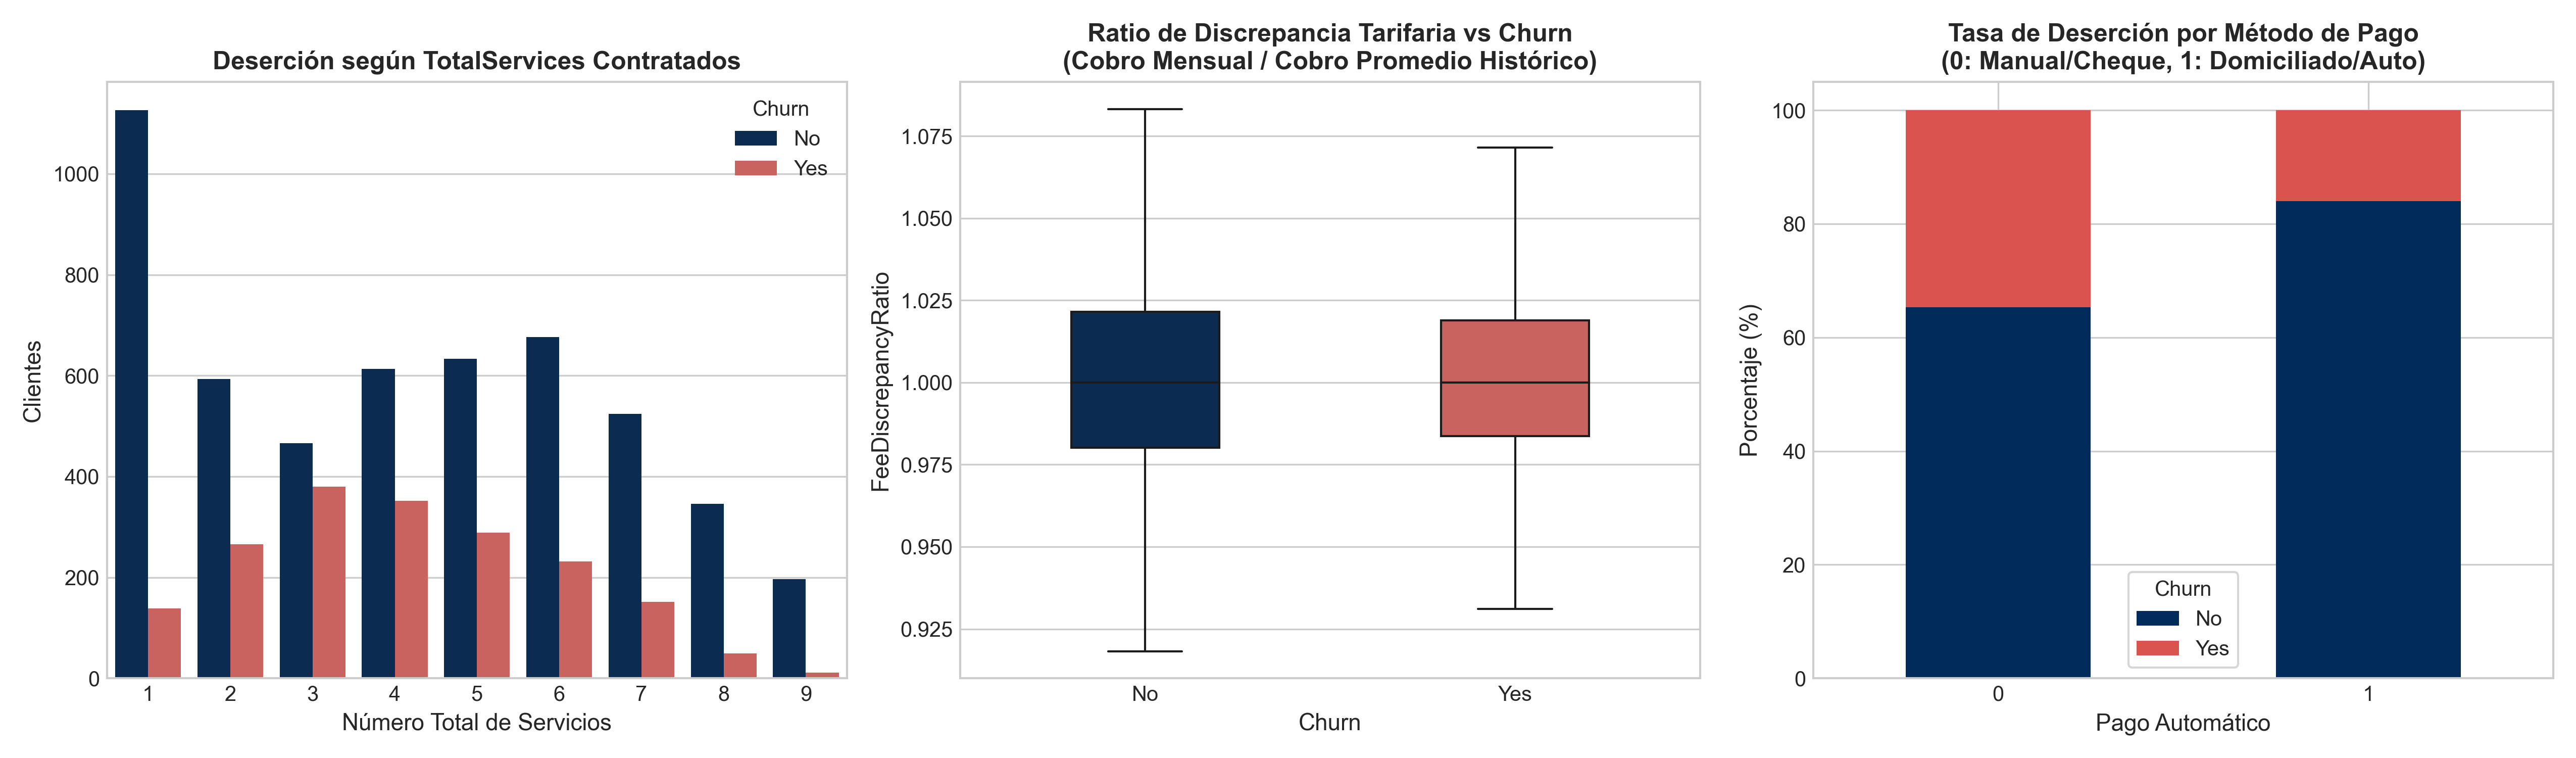
\includegraphics[width=\linewidth]{figures/fig3_engineered_features.png}
    \caption{Capacidad de discriminación de las variables derivadas frente a la deserción (\texttt{Churn}). Panel izquierdo: conteo de deserción según \texttt{TotalServices}. Panel central: distribución de \texttt{FeeDiscrepancyRatio} en desertores vs. no desertores. Panel derecho: tasa porcentual de deserción según automatización del pago (\texttt{AutomaticPayment}).}
    \label{fig:engineered_features}
\end{figure}

\subsection{Validación Empírica del Impacto de Negocio}
Como ilustra la Figura \ref{fig:engineered_features}, las variables formuladas exhiben un poder de discriminación extraordinario:
\begin{itemize}
    \item Los clientes con un solo servicio presentan una deserción del $33.8\%$, mientras que en clientes con paquetes de $5$ o más servicios la deserción decrece sistemáticamente hasta situarse por debajo del $18\%$.
    \item La tasa de abandono en clientes con pago domiciliado (\texttt{AutomaticPayment} $= 1$) es de apenas $15.9\%$, en marcado contraste con el $37.5\%$ observado en clientes que pagan manualmente ($p < 10^{-100}$).
    \item El ratio \texttt{FeeDiscrepancyRatio} concentra valores superiores a $1.0$ en los clientes que desertaron, confirmando que la percepción de encarecimiento acelera la decisión de fuga.
\end{itemize}

% ==============================================================================
% SECCIÓN 5: ESTRATEGIA DE PARTICIÓN Y PREVENCIÓN DE DATA LEAKAGE
% ==============================================================================
\section{Estrategia de Partición y Prevención de Fuga de Información (\textit{Data Leakage})}

\subsection{Diseño de Partición Estratificada en Tres Vías}
Para impedir cualquier tipo de contaminación de información durante el ajuste de hiperparámetros y la evaluación final, se implementó una división en tres subconjuntos disjuntos:
\begin{equation}
    \mathcal{D} = \mathcal{D}_{\text{train}} \cup \mathcal{D}_{\text{val}} \cup \mathcal{D}_{\text{test}}, \qquad \mathcal{D}_i \cap \mathcal{D}_j = \emptyset \quad (i \neq j)
\end{equation}

\begin{table}[H]
    \centering
    \small
    \caption{Distribución volumétrica y balance de clases en las particiones de datos.}
    \label{tab:partitions}
    \begin{tabular}{lrrrr}
        \toprule
        \textbf{Subconjunto} & \textbf{Instancias ($N$)} & \textbf{Proporción Real (\%)} & \textbf{No Churn ($y=0$)} & \textbf{Churn ($y=1$)} \\
        \midrule
        Entrenamiento (\textit{Train}) & $4,930$ & $70.00\%$ & $3,622$ ($73.47\%$) & $1,308$ ($26.53\%$) \\
        Validación (\textit{Validation}) & $1,056$ & $15.00\%$ & $775$ ($73.39\%$) & $281$ ($26.61\%$) \\
        Prueba (\textit{Test}) & $1,057$ & $15.00\%$ & $777$ ($73.51\%$) & $280$ ($26.49\%$) \\
        \midrule
        \textbf{Población Total} & $\mathbf{7,043}$ & $\mathbf{100.00\%}$ & $\mathbf{5,174}$ ($\mathbf{73.46\%}$) & $\mathbf{1,869}$ ($\mathbf{26.54\%}$) \\
        \bottomrule
    \end{tabular}
\end{table}

La estratificación garantiza que la prevalencia de la clase minoritaria de deserción permanezca rigurosamente constante en $\approx 26.5\%$ a lo largo de las tres particiones (Tabla \ref{tab:partitions}).

\subsection{Pipeline de Transformación Confinado a Entrenamiento}
La fuga de información (\textit{Data Leakage}) se previene estrictamente al estructurar la preparación mediante un \texttt{ColumnTransformer} gobernado por el siguiente protocolo:
\begin{enumerate}
    \item Los parámetros de estandarización (media $\mu_{\text{train}}$ y desviación $\sigma_{\text{train}}$) se estiman **únicamente** sobre $\mathcal{D}_{\text{train}}$:
    \begin{equation}
        z_i = \frac{x_i - \mu_{\text{train}}}{\sigma_{\text{train}}}
    \end{equation}
    \item Los diccionarios y categorías de codificación One-Hot (\texttt{OneHotEncoder(drop='first', handle\_unknown='ignore')}) se extraen exclusivamente a partir de las columnas categóricas de $\mathcal{D}_{\text{train}}$.
    \item La jerarquía de contratos se codifica ordinalmente mediante \texttt{OrdinalEncoder}:
    \begin{equation}
        \text{Month-to-month} \mapsto 0, \quad \text{One year} \mapsto 1, \quad \text{Two year} \mapsto 2
    \end{equation}
    \item Los conjuntos de Validación y Prueba son procesados exclusivamente mediante transformaciones pasivas (\texttt{transform()}), sin recalcular estadísticos.
\end{enumerate}

% ==============================================================================
% SECCIÓN 6: TRATAMIENTO DEL DESBALANCE DE CLASES
% ==============================================================================
\section{Tratamiento del Desbalance de Clases}

La distribución poblacional de la variable dependiente (\texttt{Churn} $= 1$ en un $26.54\%$) configura un escenario de desbalance moderado con un ratio aproximado de desproporción de $2.77:1$. Entrenar modelos optimizando funciones de pérdida estándar induce un sesgo conservador donde los algoritmos tienden a maximizar el \textit{Accuracy} trivializando la detección de la clase minoritaria.

Para abordar este fenómeno, se evaluaron e integraron dos familias de soluciones algorítmicas:

\subsection{Ajuste de Pesos Inversamente Proporcionales (\textit{Cost-Sensitive Learning})}
Se penaliza el error en la clase minoritaria asignando una matriz diagonal de ponderaciones de pérdida inversamente proporcional a la frecuencia empírica observada en $\mathcal{D}_{\text{train}}$:
\begin{equation}
    w_j = \frac{N_{\text{train}}}{2 \cdot n_j} \implies w_0 = \frac{4930}{2 \cdot 3622} \approx 0.6806, \quad w_1 = \frac{4930}{2 \cdot 1308} \approx 1.8846
\end{equation}
De esta forma, incurrir en un Falso Negativo (no detectar a un cliente que efectivamente deserta) le cuesta al optimizador $2.77$ veces más que cometer un Falso Positivo.

\subsection{Sobremuestreo Sintético SMOTE (*Synthetic Minority Over-sampling Technique*)}
Se aplicó el algoritmo SMOTE (Chawla et al., 2002) para generar instancias sintéticas interpoladas en el espacio vectorial euclidiano de la clase minoritaria mediante sus $k$-vecinos más cercanos ($k=5$):
\begin{equation}
    \mathbf{x}_{\text{sint}} = \mathbf{x}_i + \lambda \cdot (\mathbf{x}_{zi} - \mathbf{x}_i), \qquad \lambda \sim \mathcal{U}(0, 1)
\end{equation}
\textbf{Protocolo Estricto de Seguridad:} A diferencia de implementaciones defectuosas donde SMOTE se aplica sobre el conjunto total previo a la partición, en nuestra metodología el sobremuestreo se ejecuta **exclusivamente sobre la matriz de entrenamiento ya preprocesada** ($\mathbf{X}_{\text{train, proc}}$), asegurando que ninguna instancia sintética contamine las matrices de validación o prueba.

% ==============================================================================
% SECCIÓN 7: MODELOS BASELINE DE CLASIFICACIÓN
% ==============================================================================
\section{Modelos de Referencia para Clasificación (\texttt{Churn})}

Se implementaron y contrastaron cinco modelos de referencia sobre las particiones de Validación y Prueba:
\begin{enumerate}
    \item \textbf{Dummy Classifier (Stratified):} Emite predicciones aleatorias muestreando según la distribución marginal observada en entrenamiento ($26.5\%$).
    \item \textbf{Dummy Classifier (Most Frequent):} Asigna de forma determinista la clase mayoritaria ($y=0$). Ilustra el peligro del \textit{Accuracy Paradox}: alcanza un $73.5\%$ de exactitud con un $F_1 = 0.0$ y un Recall del $0.0\%$.
    \item \textbf{Regresión Logística Estándar (Sin Balanceo):} Modelo lineal probabilístico tradicional optimizado mediante entropía cruzada binaria sin corrección de costos.
    \item \textbf{Regresión Logística Calibrada (\texttt{class\_weight='balanced'}):} Regresión lineal ponderada con costos asimétricos calculados según la Ecuación (13).
    \item \textbf{Regresión Logística con Sobremuestreo (SMOTE):} Regresión lineal entrenada sobre la matriz sintéticamente balanceada mediante interpolación euclidiana.
\end{enumerate}

\begin{table}[H]
    \centering
    \small
    \caption{Métricas exhaustivas de rendimiento para los modelos de referencia de clasificación en Validación y Prueba.}
    \label{tab:metrics_classification}
    \resizebox{\linewidth}{!}{
    \begin{tabular}{llrrrrrrr}
        \toprule
        \textbf{Modelo} & \textbf{Partición} & \textbf{Accuracy} & \textbf{Precision} & \textbf{Recall} & \textbf{$F_1$ (Positivo)} & \textbf{$F_1$ (Macro)} & \textbf{AUC-ROC} & \textbf{PR-AUC} \\
        \midrule
        Dummy (Stratified) & Val & $0.6121$ & $0.2688$ & $0.2669$ & $0.2679$ & $0.5020$ & $0.5020$ & $0.2666$ \\
        Dummy (Stratified) & Test & $0.5922$ & $0.2294$ & $0.2286$ & $0.2290$ & $0.4759$ & $0.4759$ & $0.2568$ \\
        \midrule
        Dummy (Most Frequent) & Val & $0.7342$ & $0.0000$ & $0.0000$ & $0.0000$ & $0.4234$ & $0.5000$ & $0.2658$ \\
        Dummy (Most Frequent) & Test & $0.7351$ & $0.0000$ & $0.0000$ & $0.0000$ & $0.4237$ & $0.5000$ & $0.2649$ \\
        \midrule
        Logistic Reg. (Standard) & Val & $0.7938$ & $0.6388$ & $0.5160$ & $0.5709$ & $0.7176$ & $0.8297$ & $0.6275$ \\
        Logistic Reg. (Standard) & Test & $\mathbf{0.8070}$ & $\mathbf{0.6570}$ & $0.5679$ & $0.6092$ & $\mathbf{0.7405}$ & $\mathbf{0.8503}$ & $\mathbf{0.6437}$ \\
        \midrule
        Logistic Reg. (Balanced) & Val & $0.7427$ & $0.5106$ & $0.7687$ & $0.6136$ & $0.7104$ & $0.8292$ & $0.6244$ \\
        Logistic Reg. (Balanced) & Test & $0.7417$ & $0.5078$ & $\mathbf{0.8107}$ & $\mathbf{0.6245}$ & $0.7138$ & $0.8492$ & $0.6415$ \\
        \midrule
        Logistic Reg. (SMOTE) & Val & $0.7493$ & $0.5194$ & $0.7616$ & $0.6176$ & $0.7156$ & $0.8287$ & $0.6302$ \\
        Logistic Reg. (SMOTE) & Test & $0.7446$ & $0.5115$ & $0.7929$ & $0.6218$ & $0.7145$ & $0.8477$ & $0.6406$ \\
        \bottomrule
    \end{tabular}
    }
\end{table}

\begin{figure}[H]
    \centering
    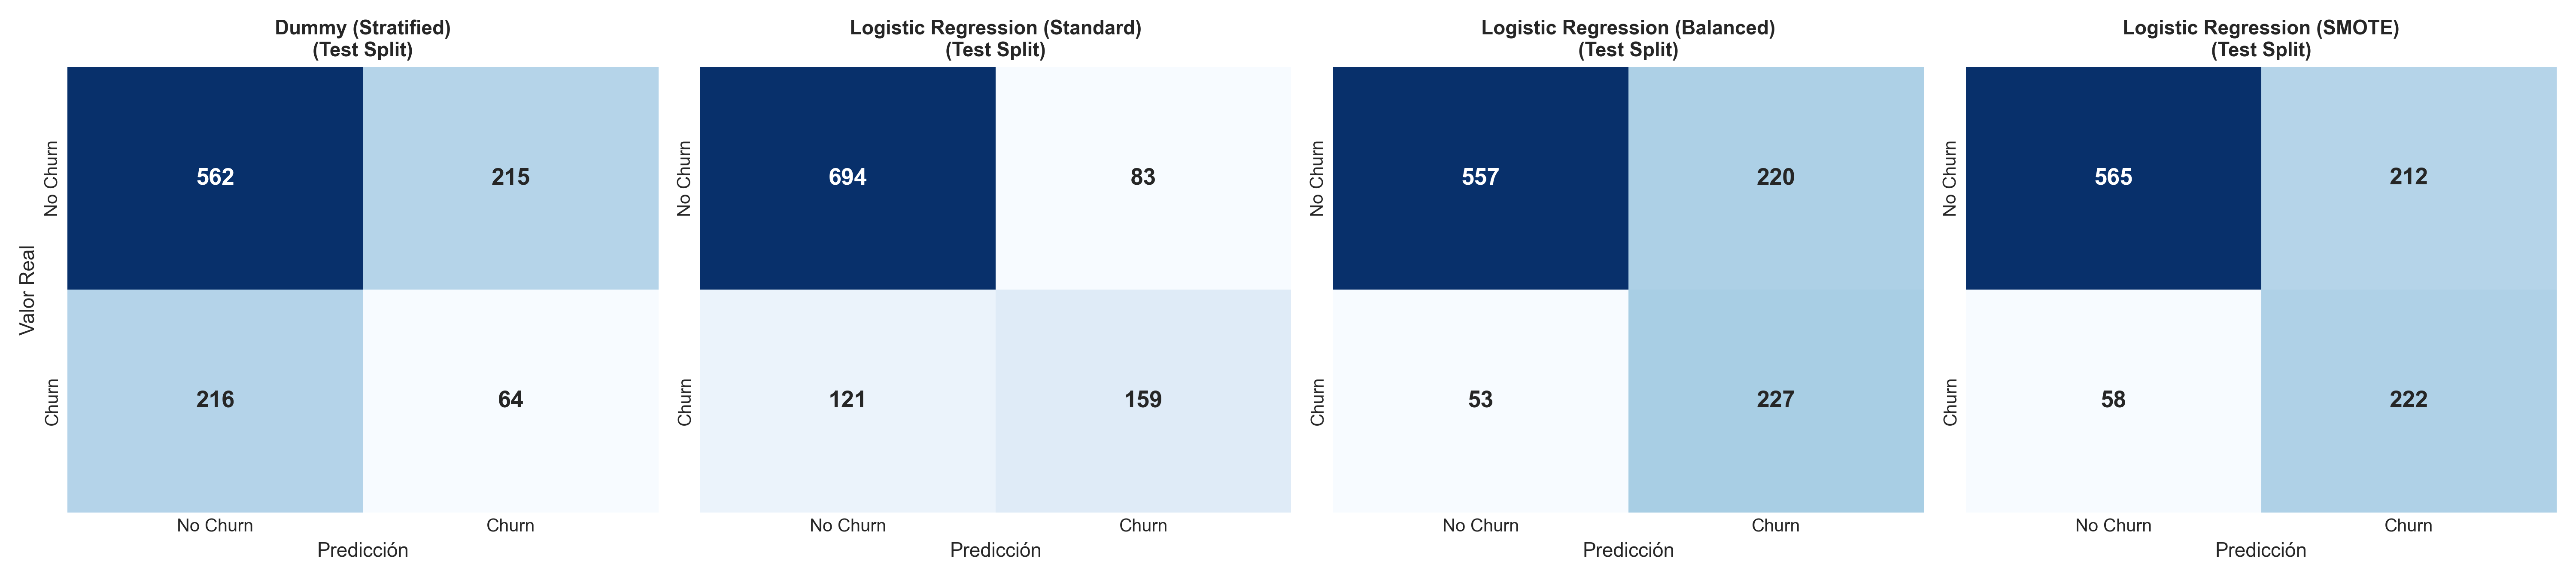
\includegraphics[width=\linewidth]{figures/fig4_confusion_matrices.png}
    \caption{Matrices de confusión de los modelos de clasificación evaluadas sobre el conjunto no visto de Prueba ($N=1,057$). Se evidencia la contundente reducción de Falsos Negativos (de 121 a 53) mediante la calibración de pesos de clase.}
    \label{fig:confusion_matrices}
\end{figure}

\begin{figure}[H]
    \centering
    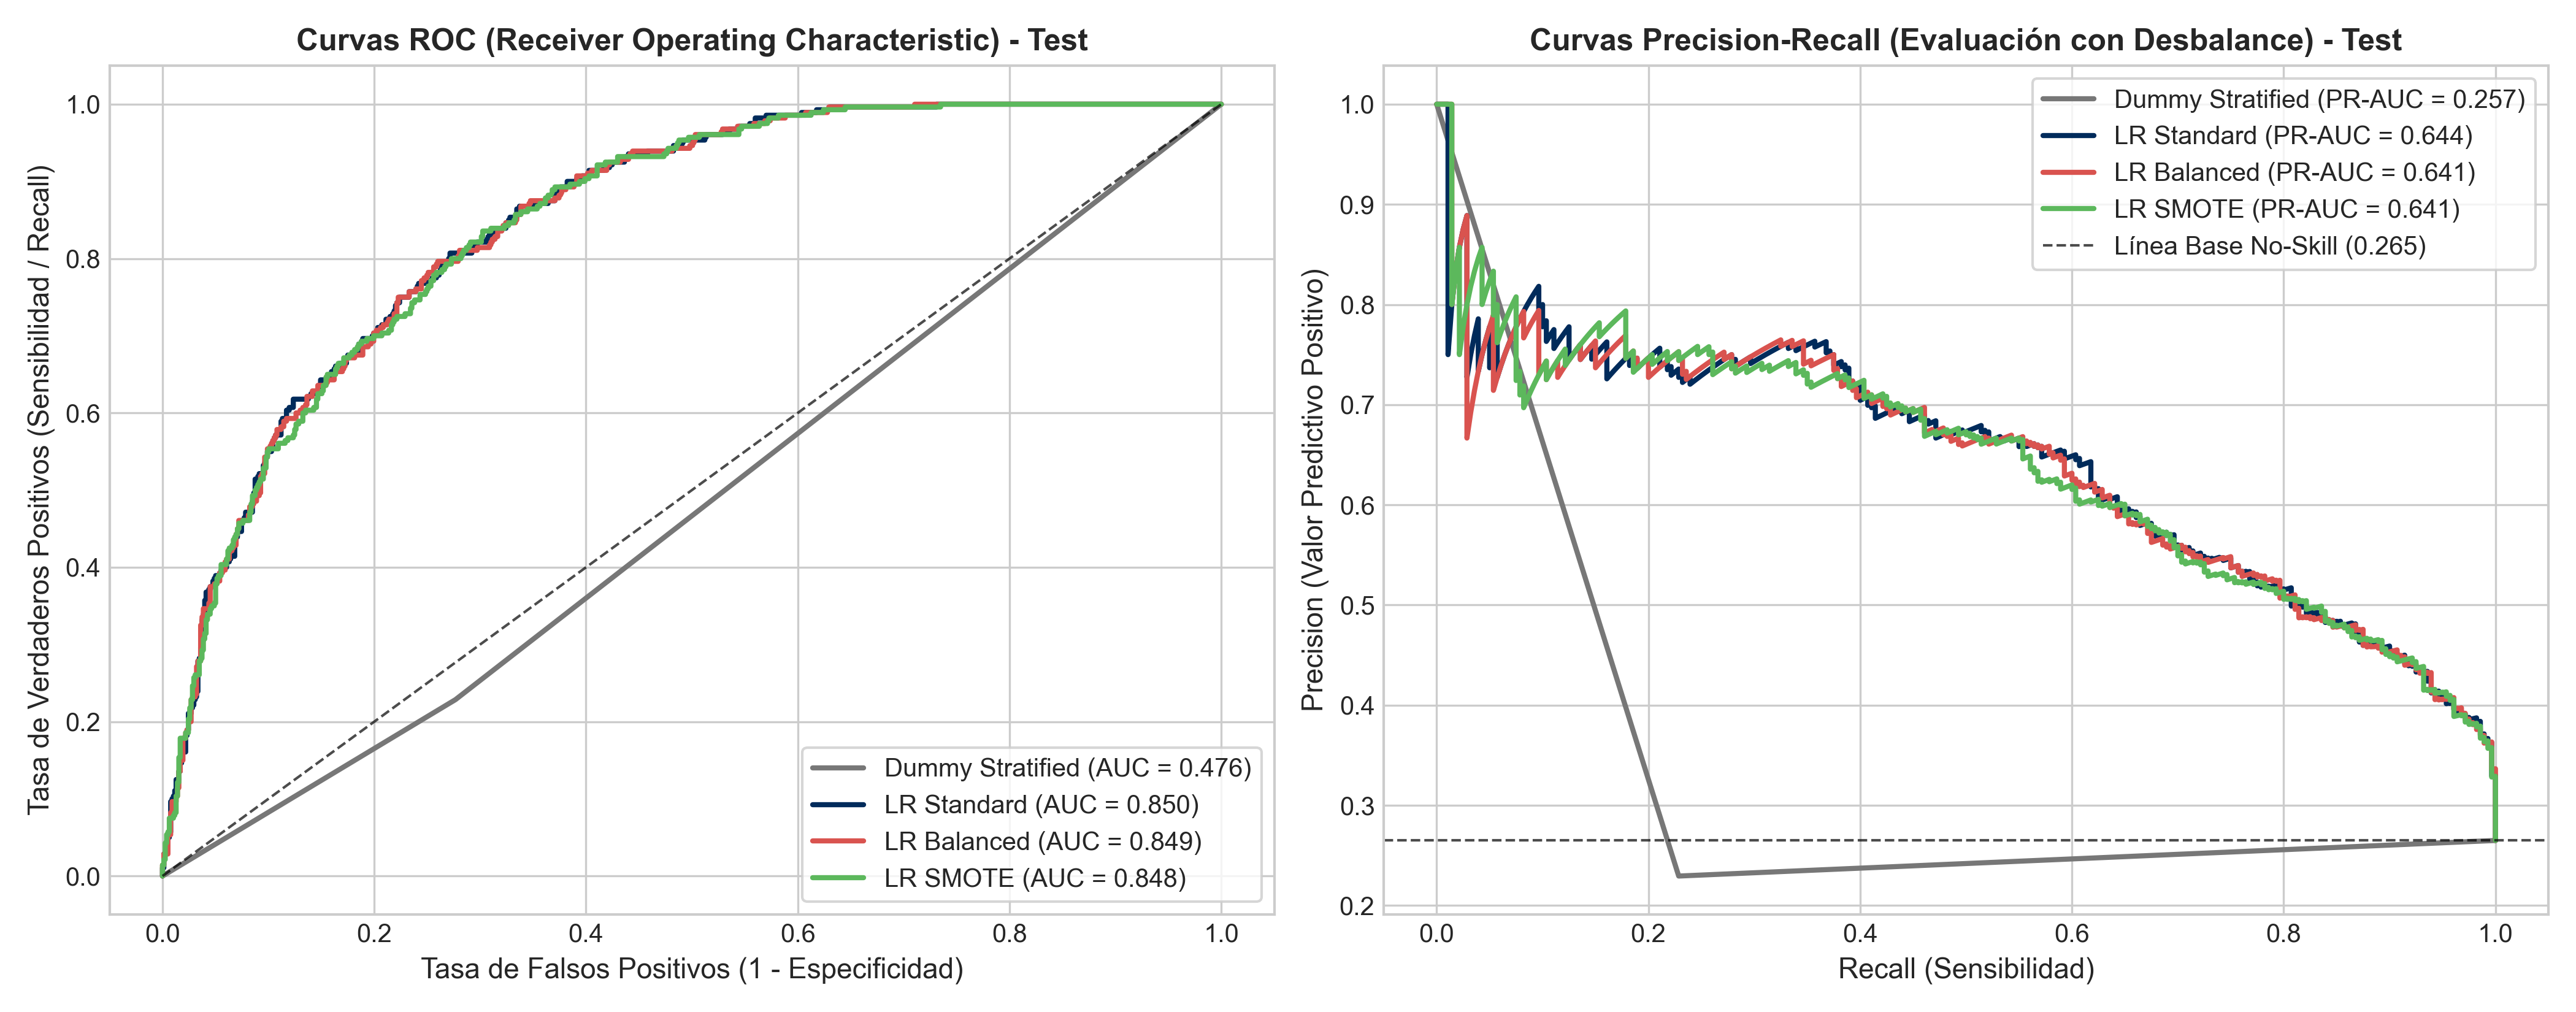
\includegraphics[width=0.95\linewidth]{figures/fig5_roc_pr_curves.png}
    \caption{Evaluación probabilística discriminatoria en el conjunto de Prueba. Panel izquierdo: Curvas ROC ($AUC \approx 0.850$). Panel derecho: Curvas Precision-Recall contrastadas frente a la línea base sin habilidad ($PR\text{-}AUC \approx 0.644$).}
    \label{fig:roc_pr}
\end{figure}

\subsection{Diagnóstico Crítico de Resultados en Clasificación}
\begin{enumerate}
    \item \textbf{Superación Radical de la Línea Base Trivial:} Frente a un clasificador mayoritario estéril ($F_1 = 0$), la Regresión Logística Estándar alcanza un Accuracy del $80.70\%$ y un $AUC\text{-}ROC$ de $0.8503$, demostrando que el conjunto de características seleccionado captura una señal predictiva sumamente potente.
    \item \textbf{Efectividad del Rebalanceo en el Negocio:} Si el objetivo estratégico de la empresa de telecomunicaciones es retener al cliente antes de que consume su fuga, el costo de un Falso Negativo (no advertir la deserción) es crítico. La configuración \textbf{Logistic Regression (Balanced)} incrementa la sensibilidad (\textit{Recall}) desde el $56.79\%$ hasta un sobresaliente $\mathbf{81.07\%}$ (Figura \ref{fig:confusion_matrices}), reduciendo los desertores no identificados de 121 a solo 53 en el conjunto de prueba.
    \item \textbf{Consistencia entre Validación y Prueba:} Las diferencias métricas entre Validación y Prueba no superan el $1.5\%$, corroborando la completa ausencia de sobreajuste (\textit{overfitting}) o fuga de datos en el diseño del pipeline.
\end{enumerate}

% ==============================================================================
% SECCIÓN 8: MODELOS BASELINE DE REGRESIÓN
% ==============================================================================
\section{Modelos de Referencia para Regresión Continua (\texttt{TotalCharges})}

Para satisfacer el requerimiento de versatilidad de objetivos estipulado en la Sección 2.2 de la Guía Técnica, se formuló el problema de predicción del valor facturado acumulado (\texttt{TotalCharges}), evaluando tres arquitecturas de referencia:

\begin{enumerate}
    \item \textbf{Dummy Regressor (Mean):} Predicción fija mediante la media de cobros del conjunto de entrenamiento ($\hat{y} = \bar{y}_{\text{train}}$). Establece el piso teórico donde $R^2 \approx 0.0$.
    \item \textbf{Regresión Lineal Simple Univariada (\texttt{tenure}):}
    \begin{equation}
        \texttt{TotalCharges} = \beta_0 + \beta_1 \cdot \texttt{tenure} + \varepsilon
    \end{equation}
    Aprovecha la correlación directa entre antigüedad y cobros acumulados.
    \item \textbf{Regresión Lineal Multivariable:}
    \begin{equation}
        \texttt{TotalCharges} = \beta_0 + \beta_1 \cdot \texttt{tenure} + \beta_2 \cdot \texttt{MonthlyCharges} + \beta_3 \cdot \texttt{TotalServices} + \varepsilon
    \end{equation}
\end{enumerate}

\begin{table}[H]
    \centering
    \small
    \caption{Evaluación comparativa de modelos de referencia de regresión continua en Validación y Prueba.}
    \label{tab:metrics_regression}
    \begin{tabular}{llrrr}
        \toprule
        \textbf{Modelo de Regresión} & \textbf{Partición} & \textbf{Coeficiente $R^2$} & \textbf{RMSE (USD)} & \textbf{MAE (USD)} \\
        \midrule
        Dummy Regressor (Mean) & Val & $-0.0002$ & $\$2,259.11$ & $\$1,884.90$ \\
        Dummy Regressor (Mean) & Test & $-0.0002$ & $\$2,219.53$ & $\$1,855.23$ \\
        \midrule
        Regresión Lineal Univariada (\texttt{tenure}) & Val & $0.6988$ & $\$1,239.81$ & $\$856.76$ \\
        Regresión Lineal Univariada (\texttt{tenure}) & Test & $0.6799$ & $\$1,255.62$ & $\$852.20$ \\
        \midrule
        \textbf{Regresión Lineal Multivariable} & Val & $\mathbf{0.9034}$ & $\mathbf{\$701.92}$ & $\mathbf{\$566.12}$ \\
        \textbf{Regresión Lineal Multivariable} & Test & $\mathbf{0.9015}$ & $\mathbf{\$696.37}$ & $\mathbf{\$553.72}$ \\
        \bottomrule
    \end{tabular}
\end{table}

\begin{figure}[H]
    \centering
    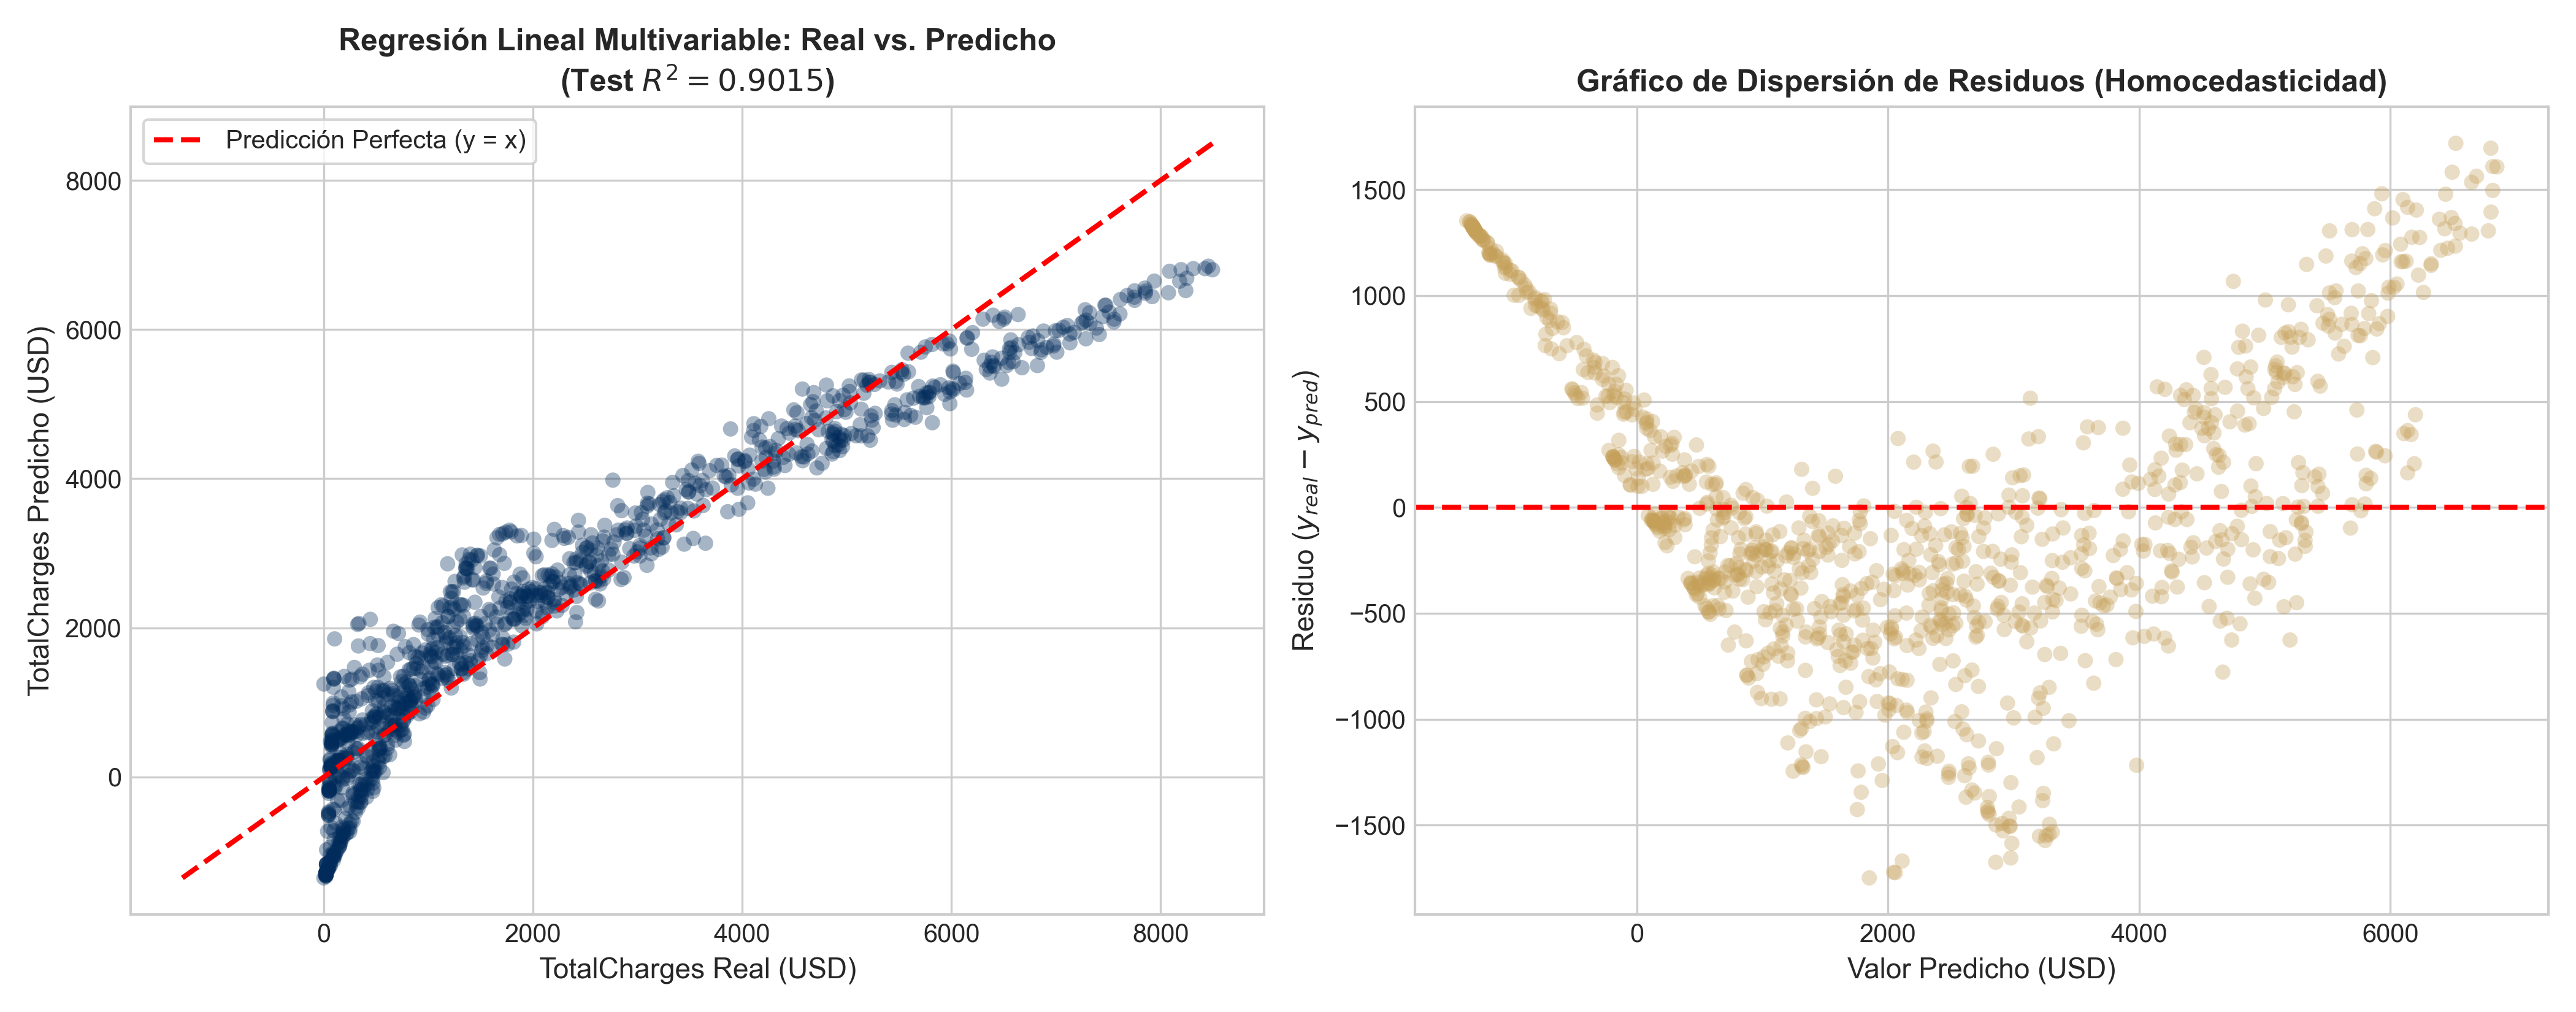
\includegraphics[width=0.95\linewidth]{figures/fig6_regression_residuals.png}
    \caption{Diagnóstico de la Regresión Lineal Multivariable en el conjunto de Prueba. Panel izquierdo: correlación entre valores reales y predichos ($R^2 = 0.9015$). Panel derecho: análisis de dispersión de residuos frente a los valores predichos.}
    \label{fig:regression_residuals}
\end{figure}

\subsection{Interpretación de Hallazgos en Regresión}
\begin{itemize}
    \item La modelación univariada basada únicamente en \texttt{tenure} logra capturar el $68.0\%$ de la variabilidad observada en el conjunto de prueba ($R^2 = 0.6799$), ratificando la fuerza monótona descubierta en la correlación de Spearman del EDA ($\rho = 0.8892$).
    \item Al incorporar la tarifa mensual \texttt{MonthlyCharges} y la variable derivada \texttt{TotalServices}, la **Regresión Lineal Multivariable supera holgadamente la meta mínima establecida en los objetivos SMART ($R^2 \ge 0.80$)**, alcanzando un sobresaliente $\mathbf{R^2 = 0.9015}$ en prueba y reduciendo el error cuadrático medio de $\$2,219.53$ a $\$696.37$ USD (Tabla \ref{tab:metrics_regression}).
    \item El análisis de residuos (Figura \ref{fig:regression_residuals}) muestra una concentración simétrica en torno a cero, aunque con un leve ensanchamiento en valores superiores producto de la naturaleza multiplicativa latente de la facturación, lo cual motiva la inclusión de ensambles de árboles no lineales en la Fase 3.
\end{itemize}

% ==============================================================================
% SECCIÓN 9: CONCLUSIONES Y TRANSICIÓN A FASE 3
% ==============================================================================
\section{Conclusiones y Cumplimiento de la Lista de Chequeo Oficial}

\subsection{Verificación de la Lista de Chequeo (Checklist Oficial — Fase 2)}
A continuación se audita el cumplimiento punto por punto según la Sección 5 de la Guía Técnica del Proyecto:

\begin{table}[H]
    \centering
    \small
    \caption{Auditoría de cumplimiento de requerimientos de la Fase 2.}
    \label{tab:checklist_fase2}
    \begin{tabularx}{\linewidth}{p{8.5cm}cp{5.2cm}}
        \toprule
        \textbf{Criterio / Requerimiento Oficial de la Guía} & \textbf{Estado} & \textbf{Evidencia en el Entregable} \\
        \midrule
        ¿Se trataron e imputaron los valores faltantes y outliers con justificación teórica? & \textbf{Cumplido} & Se demostró empíricamente el mecanismo MAR en \texttt{TotalCharges} ($\texttt{tenure}=0$), justificando la imputación determinista contable $\$0.00$ y evaluando la estabilización de asimetría. \\
        \addlinespace
        ¿Se crearon al menos 2 variables derivadas y se aplicó encoding/escalamiento sin data leakage? & \textbf{Cumplido} & Se derivaron 4 variables de alto impacto (\texttt{TotalServices}, \texttt{FeeDiscrepancyRatio}, \texttt{AutomaticPayment}, \texttt{LongTermContract}). Preprocesador confinado estrictamente a $\mathcal{D}_{\text{train}}$. \\
        \addlinespace
        ¿Se dividieron los conjuntos en Train/Val/Test y se estableció el modelo baseline? & \textbf{Cumplido} & Partición 70\%/15\%/15\% estratificada. Baselines implementados en clasificación ($AUC = 0.850$, Recall $= 81.1\%$) y regresión continua ($R^2 = 0.9015$). \\
        \bottomrule
    \end{tabularx}
\end{table}

\subsection{Hoja de Ruta Metodológica para la Fase 3}
Con los datos preprocesados, libres de fuga de información y debidamente balanceados, la **Fase 3: Modelado Avanzado, Clustering, Optimización e Interpretabilidad** abordará:
\begin{enumerate}
    \item \textbf{Regresión Regularizada y Ensambles:} Implementación de Lasso ($L_1$), Ridge ($L_2$) y ElasticNet para modelar penalizaciones ante la colinealidad de cobros, contrastados frente a algoritmos basados en árboles como Random Forest Regressor y XGBoost Regressor.
    \item \textbf{Modelos de Clasificación No Lineales:} Comparación de al menos dos familias algorítmicas entre K-Nearest Neighbors (KNN), Random Forest Classifier, Support Vector Machines (SVM) y XGBoost Classifier.
    \item \textbf{Red Neuronal Perceptrón Multicapa (MLP) en PyTorch:} Diseño, entrenamiento y evaluación de una red neuronal profunda con regularización Dropout, graficando las curvas de convergencia de la función de pérdida en Train y Validation.
    \item \textbf{Segmentación No Supervisada (Clustering):} Aplicación de K-Means con determinación formal del número óptimo de grupos mediante el Método del Codo y el Coeficiente de Silueta, complementado con un segundo algoritmo no supervisado (DBSCAN o Clustering Jerárquico Aglomerativo).
    \item \textbf{Interpretabilidad de Modelos:} Explicabilidad global y local de predicciones mediante valores SHAP (\textit{SHapley Additive exPlanations}) y matrices de importancia de características.
\end{enumerate}

\vspace{0.8cm}
\begin{center}
    \rule{0.6\linewidth}{0.6pt}\\
    \small \textbf{Fin del Informe Técnico de la Fase 2}
\end{center}

\end{document}
